\documentclass[12pt,twocolumn]{article} 
\usepackage[utf8]{inputenc} 
\usepackage[margin=.75in,nohead,nofoot]{geometry}
\usepackage{graphicx} 
\usepackage{epstopdf} 
\usepackage{amsfonts}
\usepackage{amssymb}
\usepackage{amsmath}
% \usepackage[parfill]{parskip} % Activate to begin paragraphs with an empty line rather than an indent

\def\avg#1{\langle#1\rangle}
\def\v#1{\mathbf{#1}}
\def\Re {\mbox{Re}}
\def\Im {\mbox{Im}}
\def\tr{\mbox{tr}}
\def\nn{\nonumber}
\def\pp{\parallel}
\def\ket#1{\vert #1 \rangle}
\def\bra#1{\langle #1 \vert}
\def\me#1#2#3{\langle #1 \vert #2 \vert #3 \rangle}
\def\Br{\mathbf{r}}

\newcommand{\kp}{k_{+}}
\newcommand{\ki}{k_{-}}
\newcommand{\idz}{i\partial_z}
\newcommand{\kperp}{\mathbf{k}_\parallel}


\linespread{1.1}

\title{Mesoscopic studies of Topological Insulators and Superconductors\\Mahmoud Lababidi}
\author{Mahmoud Lababidi}
\date{}

\begin{document}
\maketitle

\section*{Overview/Forward}
In this proposal I will have four basic parts that break down the why, how and what I propose to do in my research for my thesis. I begin by presenting a brief introduction to topological insulators which can be skipped for brevity if one is already familiar with the subject. This introduction will not be as detailed as many papers on the subject but should suffice for understanding the proposed actions in this letter. Then I will highlight some novel and interesting physics that have been spurred from the TI. This is simply to motivate the projects that I have and will work on. Next, I will present work already completed and in progress. Lastly, I will present the next projects that I aim to complete towards my research. 


\subsection*{Introduction/Background}
Topological Insulators (TIs) are a new form of matter that have robust conducting metallic surface states while the bulk is an insulator. The surface is so vastly different from the bulk, that it can be seen as a playground of new properties never seen before. One such novel property is that the surface is host to Dirac Fermions which behave relativistically and massless-like. Such particle behavior was predicted by Paul Dirac. The first experiment that demonstrated this prediction was done on graphene, a very similar cousin to the TI. These particles are identified as  Dirac Fermions because they obey the Dirac equation which models relativistic (near speed of light) particles. These massless relativistic Fermions, demonstrate a direct linear relationship between the energy (E) and their quantized momentum (k), $E=\pm\hbar v k$. This peculiar energy relationship is uncommon in  materials. 

TIs have gained much notoriety for a variety of new physics. Such physics include the proposal to generate Majorana particles, which are non-Abelian, through the use of superconductors in proximity; interesting conductance on the surface due to the Dirac-like Hamiltonian and spin (eg Klein Tunneling); and the possibility of new topological phases of materials.




\subsection*{Spintronics}

\clearpage


\subsection*{Robustness of single-qubit geometric gate against systematic error}
The third paper involves a calculation takes a clever approach to manipulate a quantum system and compares it to a traditional approach of quantum control. The paper shows that the new approach is more robust to systematic and random errors than the traditional approach using a quantitative metric called quantum fidelity. Such a result has great implications in quantum control and in turn quantum computing, the holy grail of information science.

\subsection*{Current Work}
In continuation of my previous work, I have studied superconductors in close proximity to TIs. As stated in the previous section, the implications are vast and many interesting experiments can be performed to understand new physics with such a class of materials. Currently there are three projects that are near completion. The first project is the study of the proximity effect on the surface of the TI and a superconductor. This project differs greatly from the second paper because in the second paper, the primary focus was not directed at the surface but rather, the inner bulk of the TI. Material-wise we model Bi$_2$Se$_3$. One key result from this is the local density of states (LDOS) (figure b.) shows a second smaller bump forming due to the TI, which is an anomalous effect when compared to traditional superconductors (see high peak red plot in figure b.). This second bump is an important signature of a new type of superconductivity that is unconventional. 

The second project is the Josephson $\pi$ junction on the surface of the TI. This setup was predicted to host Majorana particles but no one has performed a realistic, self consistent simulation. The results provide information about the zero-energy Majorana. Figure a.shows the zero-energy crossings that are the signatures of the Majorana. The TI surface, when in contact with a superconductor, can host the elusive Majorana particle. One of the signatures of the Majorana is the zero energy, which can be seen in figure a. where the graph has intersection points at E=0. 


The third project involves calculating the conductance of a TI  and superconductor junction where the results differ greatly from the traditional Blonder-Tinkham-Klapwijk theory for conductance. 

\clearpage
\section{Future Work}
\section{Josephson Pi Junction}
It has been proposed and discussed that by placing an s wave superconductor in proximity with the surface of a TI, the surface interface under certain circumstances can be host to Majorana particles. These circumstances incluce the following: a Josephson junction on the surface of the TI where the complex phase angle difference between the two superconducting leads is $\pi$, a vortex on the interface surface where the complex phase angle winds by $2 \pi$ around the core/center, a magnetic domain wall where the magnetic fields of the two sides of the junction are pointing in opposite directions. [maybe drawings?, needs refs]

The first two of these proposals llow us to study very similar physics due to the following argument. The $\pi$ phase difference found in a Josephson junction is found in superconducting vortex where the complex phase angle difference between one side of the core to the opposite side is also $\pi$. Though the similarities between the two structures are seen in this light, this is not to discount the vortex proposal because of possible new rich physics that can be discovered. One example of such physics could be due to the topology of the structure such as along the outer edge vortex boundary, which a $p_x+i p_y$ superconductor (which breaks time reversal) is host to chiral edge modes. But I leave this digression for another future discussion and possible study. 

In addition to studying the $\pi$ junction, we also study the 0 phase junction as well. The zero phase junction also shows some interesting results, mainly in the local density of states where a second "gap" is produced. 

\subsection{Model}
The Hamiltonian for the Josephson junction TI surface as shown in the figure is given by the Bogoliobuv-deGennes-Dirac Hamiltonian as:

\begin{eqnarray}
&\mathcal{H}=\left(
\begin{array}{cc}
h_{+}  &  \hat{\Delta} \\
\hat{\Delta}^\dagger  &   h_{-}
\end{array}\label{fkmodel}
\right),&
\end{eqnarray}
where
\begin{eqnarray}
&h_{\pm}= -i\hbar  v_F (\sigma_x\partial_x \pm \sigma_y \partial_y) \mp \mu(x),&\\
&\hat{\Delta}= i\sigma_y  \Delta(x).&
\end{eqnarray}


\section*{MOSFET with TIs}
In the following project proposal, I present a possible electronic heterostructure that could, in theory, store multiple classical logic states. The main framework this is based upon is the "floating gate" Metal-Oxide-Silicon Field Effect Transistor (MOSFET) that is the standard in all of today's electronics. The MOSFET is a device
\section*{Non-Equilibrium Dynamics with TIs}
Once these projects are complete, there are many interesting directions to go in this world of TIs. Experiments are currently being conducted at many universities to study the many aspects of the TI. Much collaboration is available to present a lot of new physics.

The Jiang research group at Georgia Institute of Technology has conducted a few Andreev spectroscopy experiments in superconductor-TI heterostructures and reached out to us for collaboration to understand some results of their experiments. Additionally, we will study non-equilibrium physics of TIs, by modeling the TIs with an additional driving force, such as a magnetic field, an optical laser or voltage bias. There has been work in achieving a creation of a topological state similar to a TI through the use of similar driving forces. This work can give much insight into the new topological nature of matter. Lastly, I have been in talks with Qiliang Li of the Electrical and Computer Engineering department at GMU about doing calculations on a possible device built from a TI that could be used as a new form of memory. The possibility of this stems from the uncommon current-voltage relationship that the TI has. Such a device would improve efficiency in storage devices such as flash memory and essentially be a new device to complement or even replace silicon.
\begin{figure}[ht]

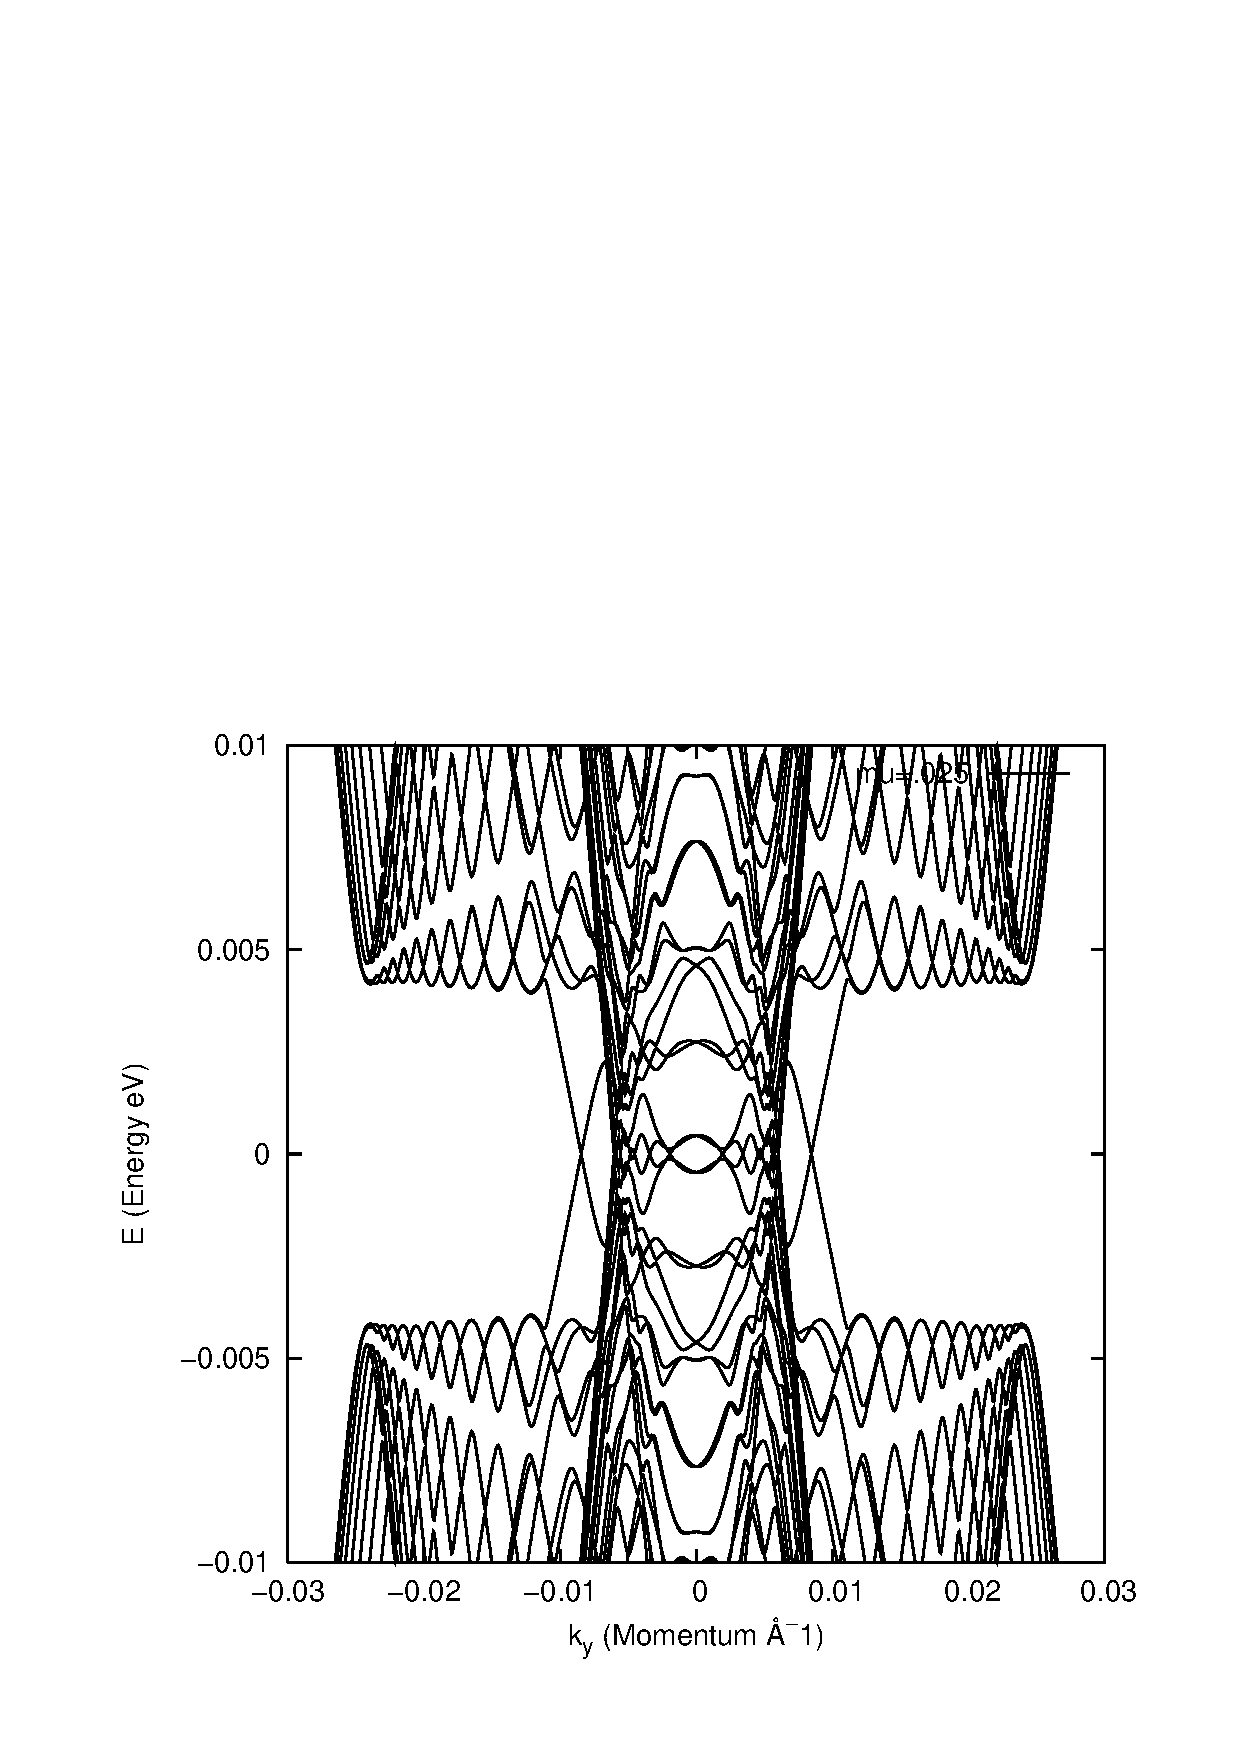
\includegraphics[width=2in]{energy_zoom}
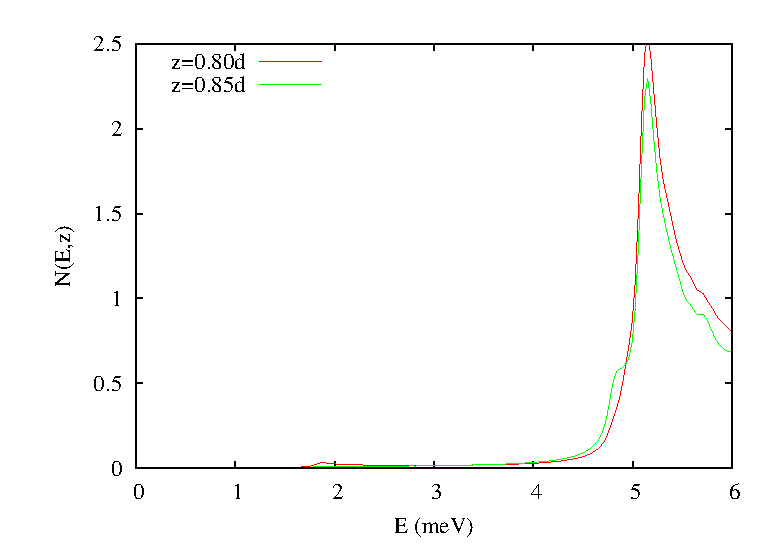
\includegraphics[width=2in]{dos}
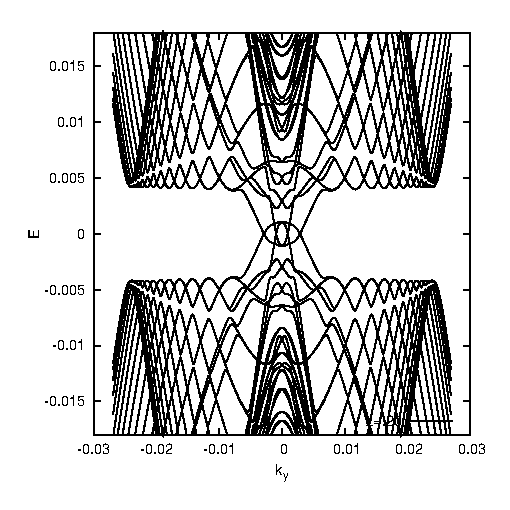
\includegraphics[width=2in]{energy_pi}
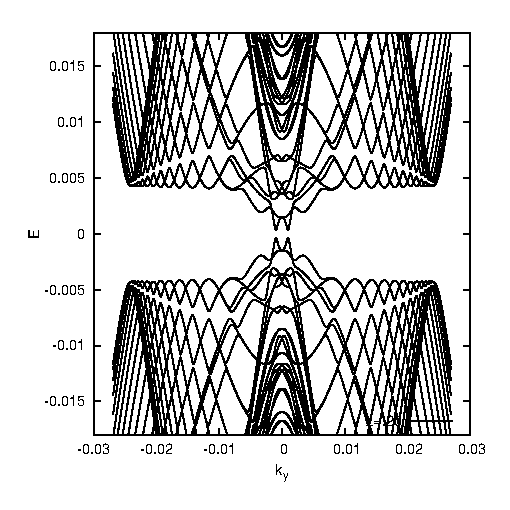
\includegraphics[width=2in]{energy_zero}

\caption{(color electronic version) a. Plotted are energies of S-TI-S Josephson $\pi$ junction on the surface. The zero-energy crossings in the plot represent possible Majorana particle states. b. Plotted is the local density of states of a S-TI-S zero-phase surface as a function of energy and position along the surface. 
}\label{setup}
\end{figure}

\end{document}


%%% PACKAGES
%\usepackage{booktabs} % for much better looking tables
%\usepackage{array} % for better arrays (eg matrices) in maths
%\usepackage{paralist} % very flexible & customisable lists (eg. enumerate/itemize, etc.)
%\usepackage{verbatim} % adds environment for commenting out blocks of text & for better verbatim
%\usepackage{subfig} % make it possible to include more than one captioned figure/table in a single float
% These packages are all incorporated in the memoir class to one degree or another...


%\setlength{\parskip}{0pt}
%\setlength{\parsep}{0pt}
%\setlength{\headsep}{0pt}
%\setlength{\topskip}{0pt}
%\addtolength{\textheight}{00pt}
%\setlength{\topmargin}{-30pt}
%\setlength{\topsep}{0pt}
%\setlength{\partopsep}{0pt}

%\usepackage[compact]{titlesec}
%\titlespacing{\section}{0pt}{*0}{*0}
%\titlespacing{\subsection}{0pt}{*0}{*0}
%\titlespacing{\subsubsection}{0pt}{*0}{*0}